\chapter{Introduction}

Unmanned Aerial Vehicles (UAVs) have seen an explosion of use in the last few decades in both civilian and defense spaces. UAVs take advantage of the vast airspace available over land, sea, and city to avoid the traffic inherent to civilization \cite{sabour2023applications}. UAVs can reach remote locations in minutes what would otherwise take hours or days for humans and automobiles to reach, such as remote or mountainous areas with poor roads. Small UAVs are performing many tasks that used to require large and expensive manned helicopters and airplanes, such as creating aerial shots in film \cite{aerial_shot} or surveying construction sites \cite{drones6050117}. As demand for this technology continues to increase, so will demand for better autopilots and controllers.

Airplanes are aircraft that generate lift using an airframe and forward airspeed. 
That is, they rely on moving quickly and using an airfoil to generate lift, and a propeller or jet engine to generate thrust.
Airplanes are very efficient at moving long distances quickly.

Rotorcraft are aircraft that generate lift solely from vertically oriented rotors. This is to say, they generate little to no lift from airflow over some sort of airfoil. Some examples of rotorcraft include helicopters, quadcopters, and hexacopters, as shown in \ref{fig:Multicopters}. Pure rotorcraft UAVs like quadcopters have several advantages over fixed-wing aircraft. They can take off and land almost anywhere without any additional hardware, while airplanes require landing strips or launch tracks. Quadcopters can also converge to and hold a set position, unlike airplanes which have to remain in motion to stay airborne. Quadcopters are more maneuverable and can track almost any trajectory, as they do not have a minimum turning radius. 

\begin{figure}[htbp]
    \centering
    \begin{subfigure}{0.48\textwidth}
        \centering
        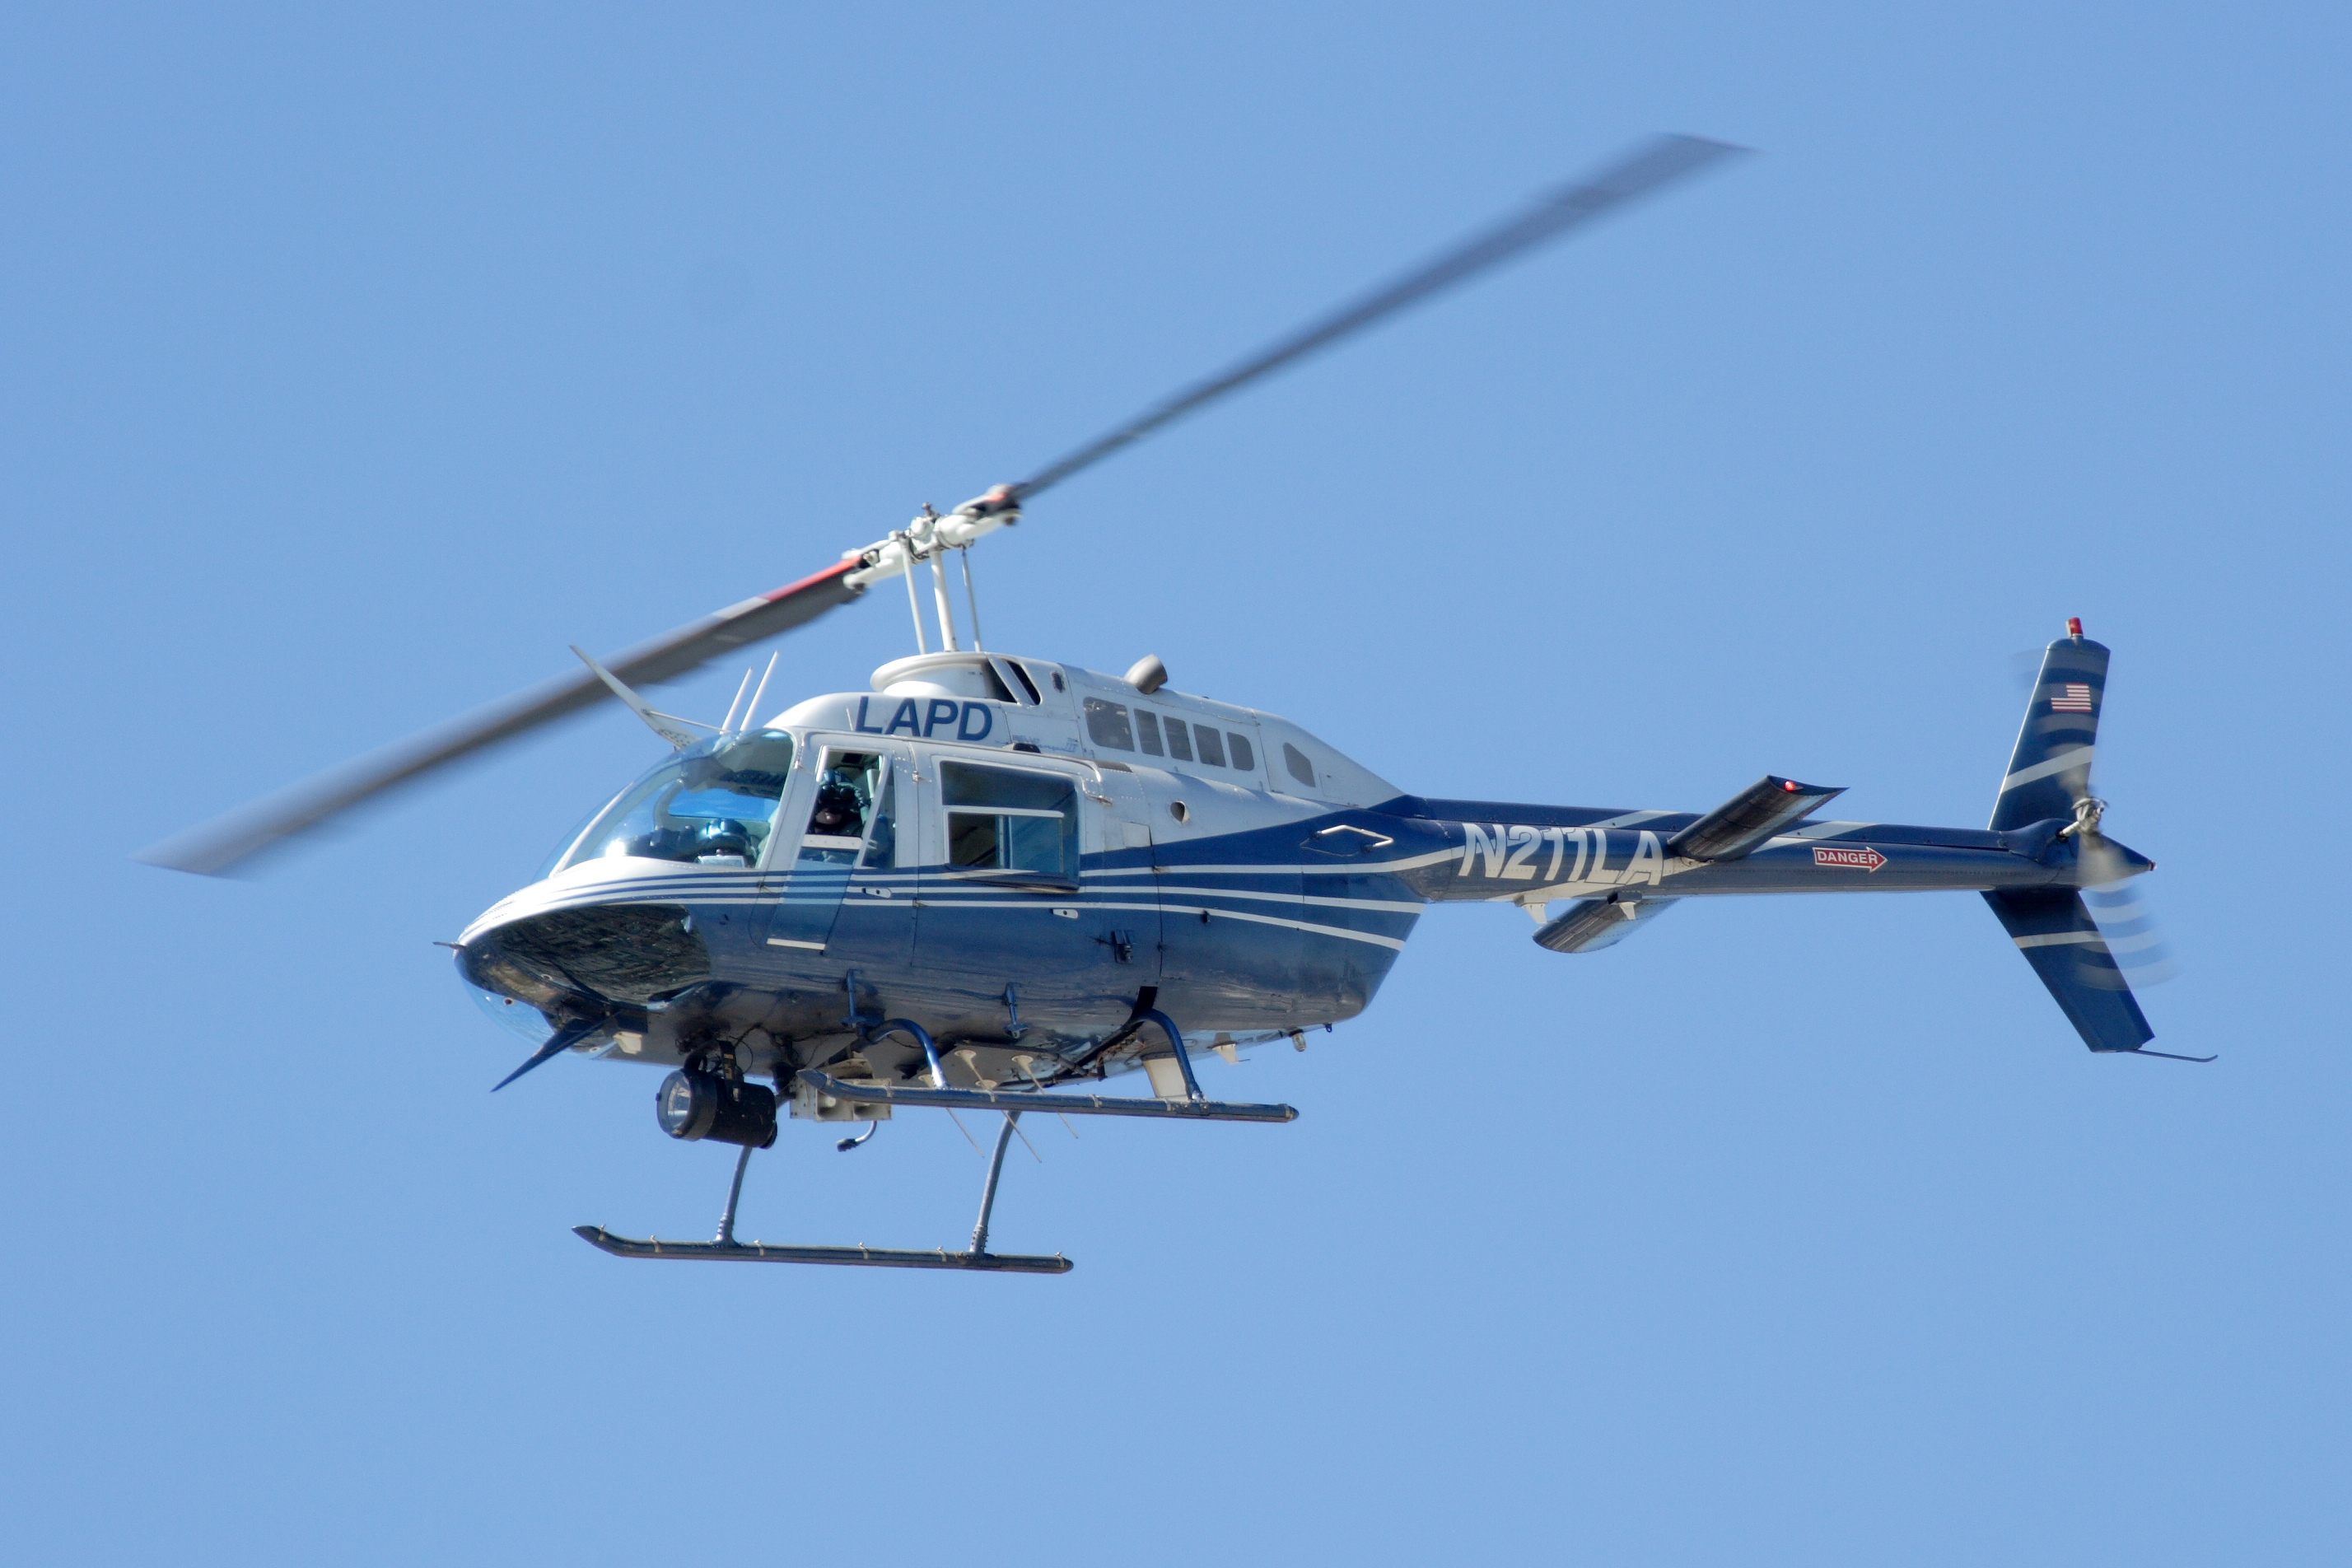
\includegraphics[width=\linewidth]{figs/chap0/LAPD_Bell_206_Jetranger.jpg}
        \caption{Los Angeles Police Department (LAPD) Bell 206 Jetranger helicopter. Photograph by Mfield – Matthew Field, 2006, via Wikimedia Commons. Licensed under Creative Commons Attribution-ShareAlike 3.0 Unported (CC BY-SA 3.0) and Creative Commons Attribution 2.5 (CC BY 2.5).\cite{lapd_bell206_jetranger}}
        \label{fig:bellJetranger}
    \end{subfigure}
    \hfill
    \begin{subfigure}{0.48\textwidth}
        \centering
        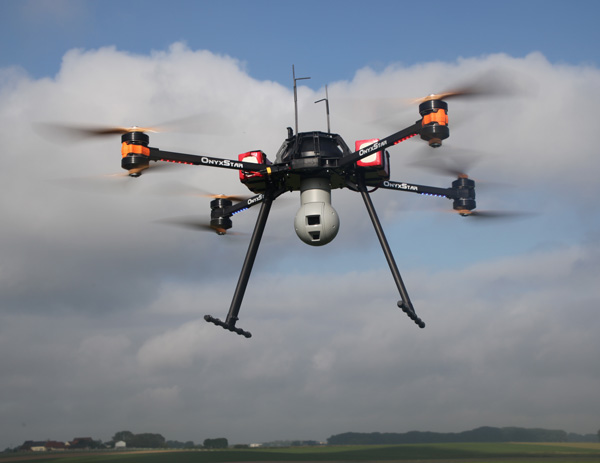
\includegraphics[width=\linewidth]{figs/chap0/Onyxstar_Fox-C8_XT_xender_360.jpg}
        \caption{Onyxstar Fox-C8 XT Xender 360 UAV. Image by ZullyC3P (2015), via Wikimedia Commons. Licensed under Creative Commons Attribution-ShareAlike 4.0 International (CC BY-SA 4.0). \cite{onyxstar_foxc8_xt_xender_360}}
        \label{fig:Onyxstar}
    \end{subfigure}

    \vspace{0.5cm}  % vertical spacing between rows

    % Row 2
    \begin{subfigure}{0.48\textwidth}
        \centering
        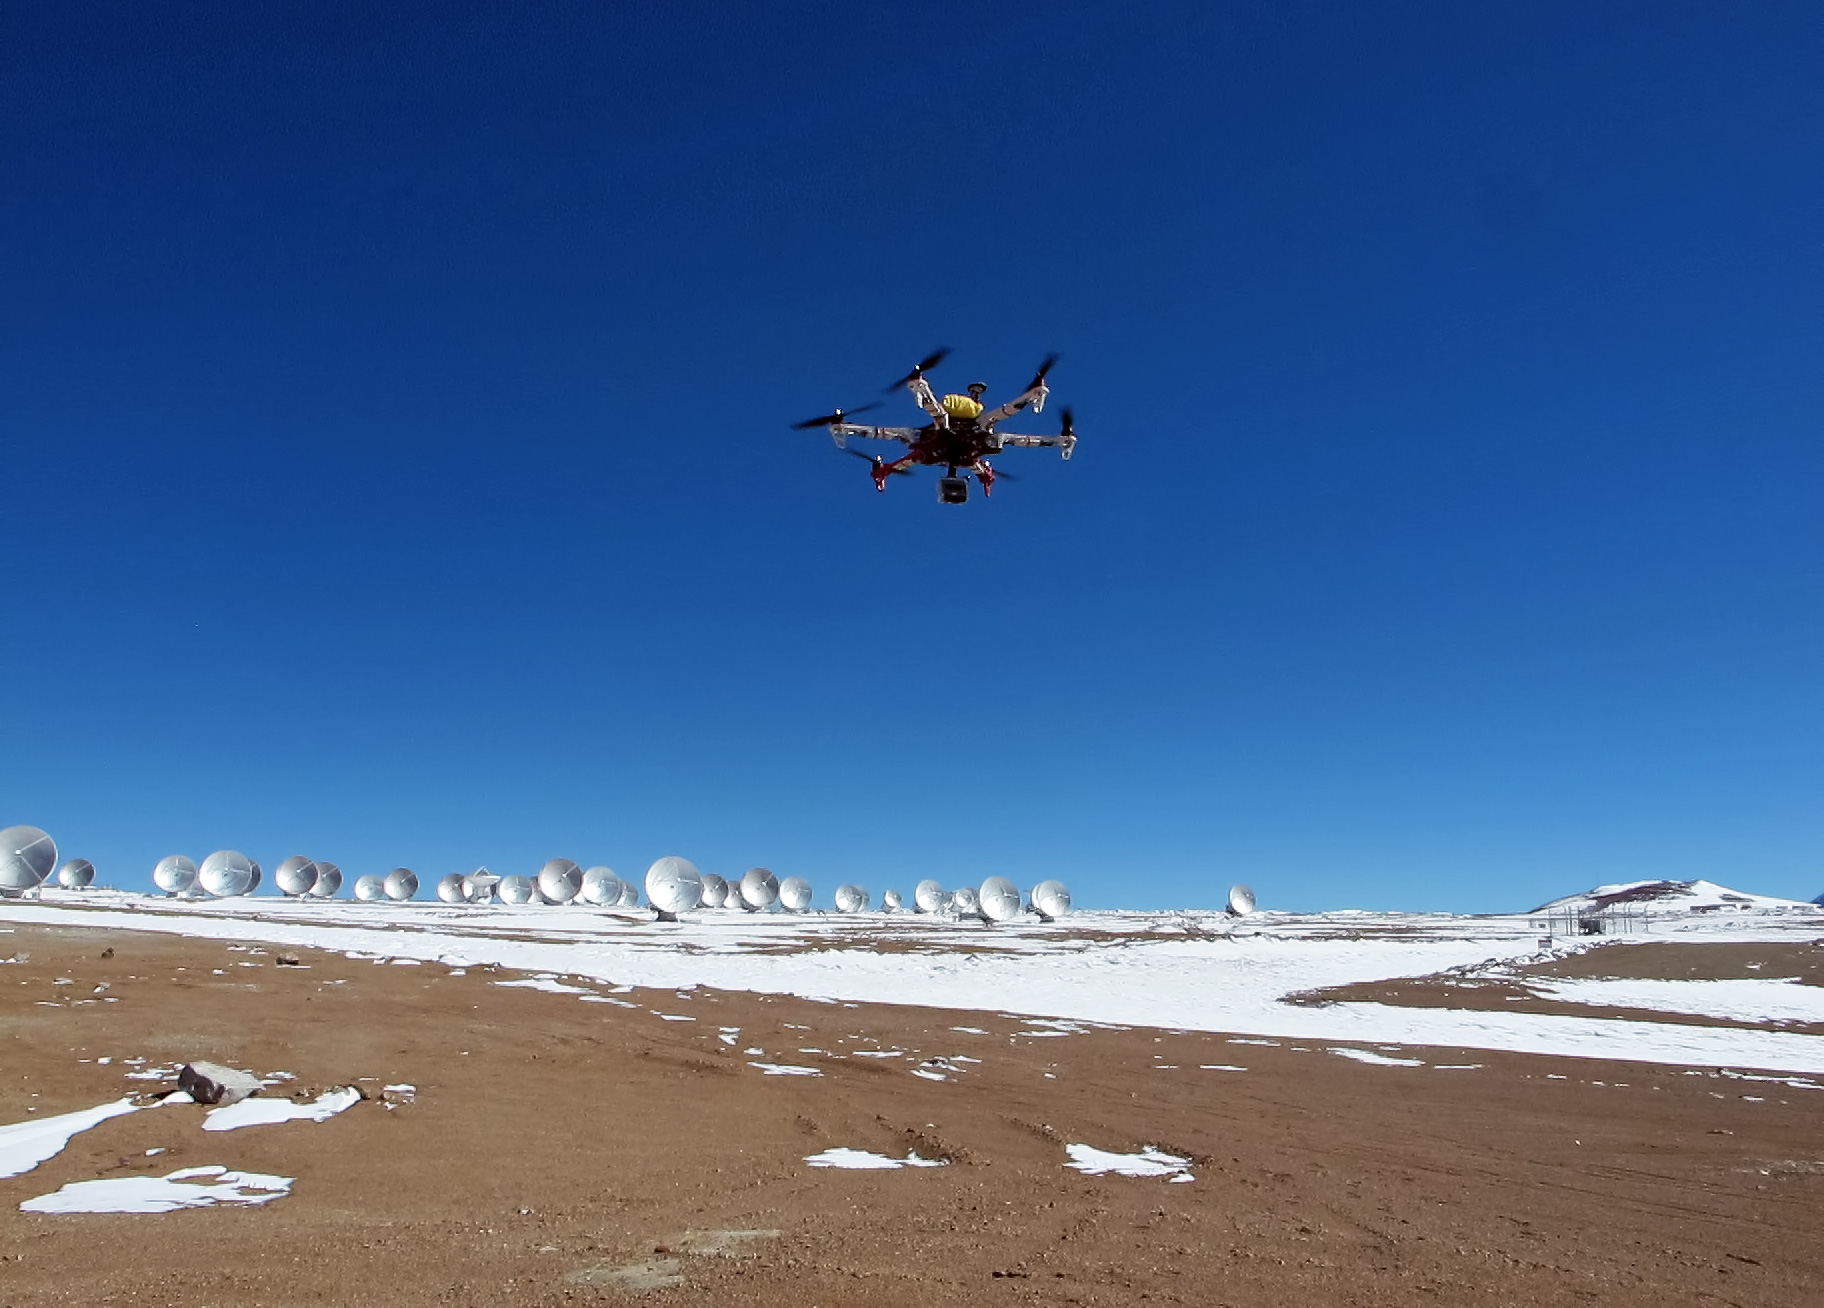
\includegraphics[width=\linewidth]{figs/chap0/The_Hexacopter.jpg}
        \caption{Hexacopter UAV with camera over the ALMA observatory. Image by ALMA (ESO/NAOJ/NRAO), 2013, via Wikimedia Commons, licensed under Creative Commons Attribution 4.0 International (CC BY 4.0). \cite{the_hexacopter}}
        \label{fig:hexacopter}
    \end{subfigure}
    \hfill
    \begin{subfigure}{0.48\textwidth}
        \centering
        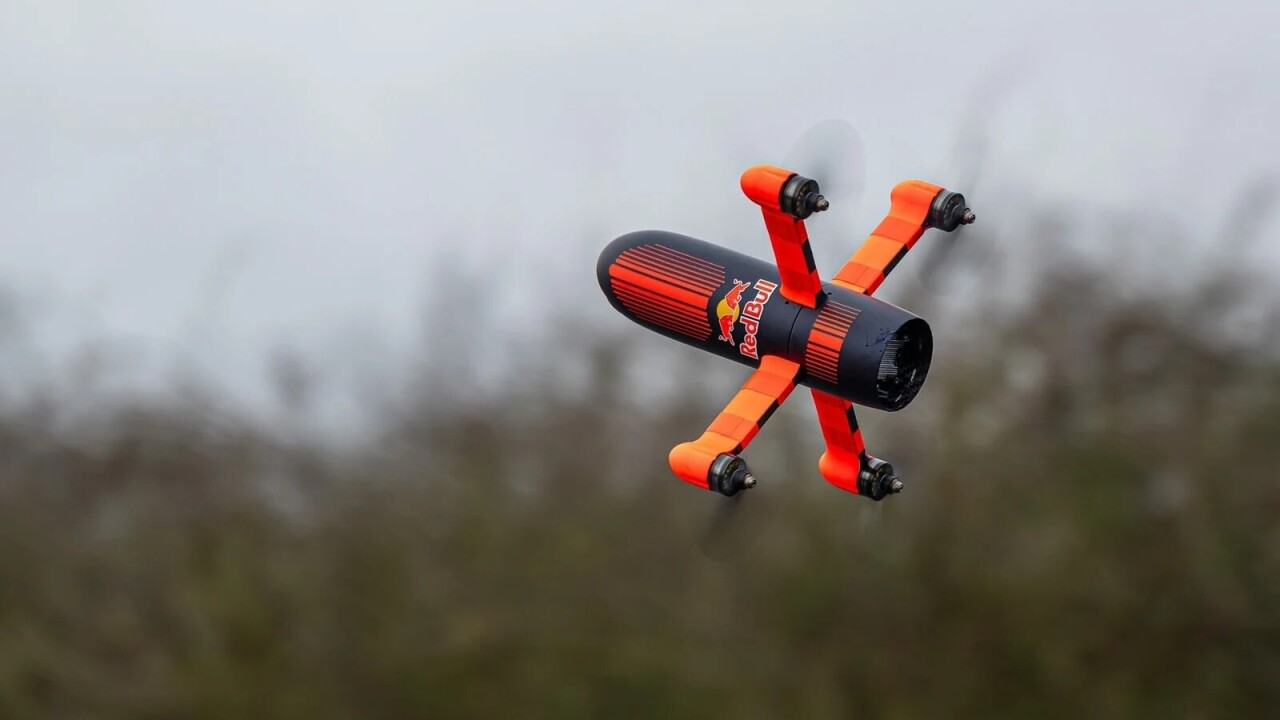
\includegraphics[width=\linewidth]{figs/chap0/redbull.jpeg}
        \caption{World’s fastest camera drone chasing Max Verstappen’s Formula 1 car, as shown in the article “Watch: World’s fastest camera drone races F1 champ Max Verstappen,” published on The Next Web (February 29, 2024). Image used under editorial rights with The Next Web. \cite{tnw_fastest_camera_drone_image}}
        \label{fig:racingDrone}
    \end{subfigure}    
    
    \caption{Four different multicopters. Fig. \ref{fig:racingDrone} is kind of a VTOL itself, due to its high vertical speed.}
    \label{fig:Multicopters}
\end{figure}

However, airplanes are much more efficient at traveling long distances at high speeds, with much less energy consumption than copters. A quadcopter uses four rotors with fairly high power consumption just to stay in the air without any movement, while an airplane uses a relatively low power thruster maintain a high kinetic energy. For a given battery size, an airplane can stay in the air significantly longer than its equivalent rotorcraft. Airplanes have fewer moving parts than rotorcraft, and can glide to safety in case of rotor failure, which lends some inherent advantages to the use of airframes. Some examples of fixed wing UAVs are shown in Fig. \ref{fig:FixedWings}.

\begin{figure}[htbp]
    \centering
    \begin{subfigure}{0.48\textwidth}
        \centering
        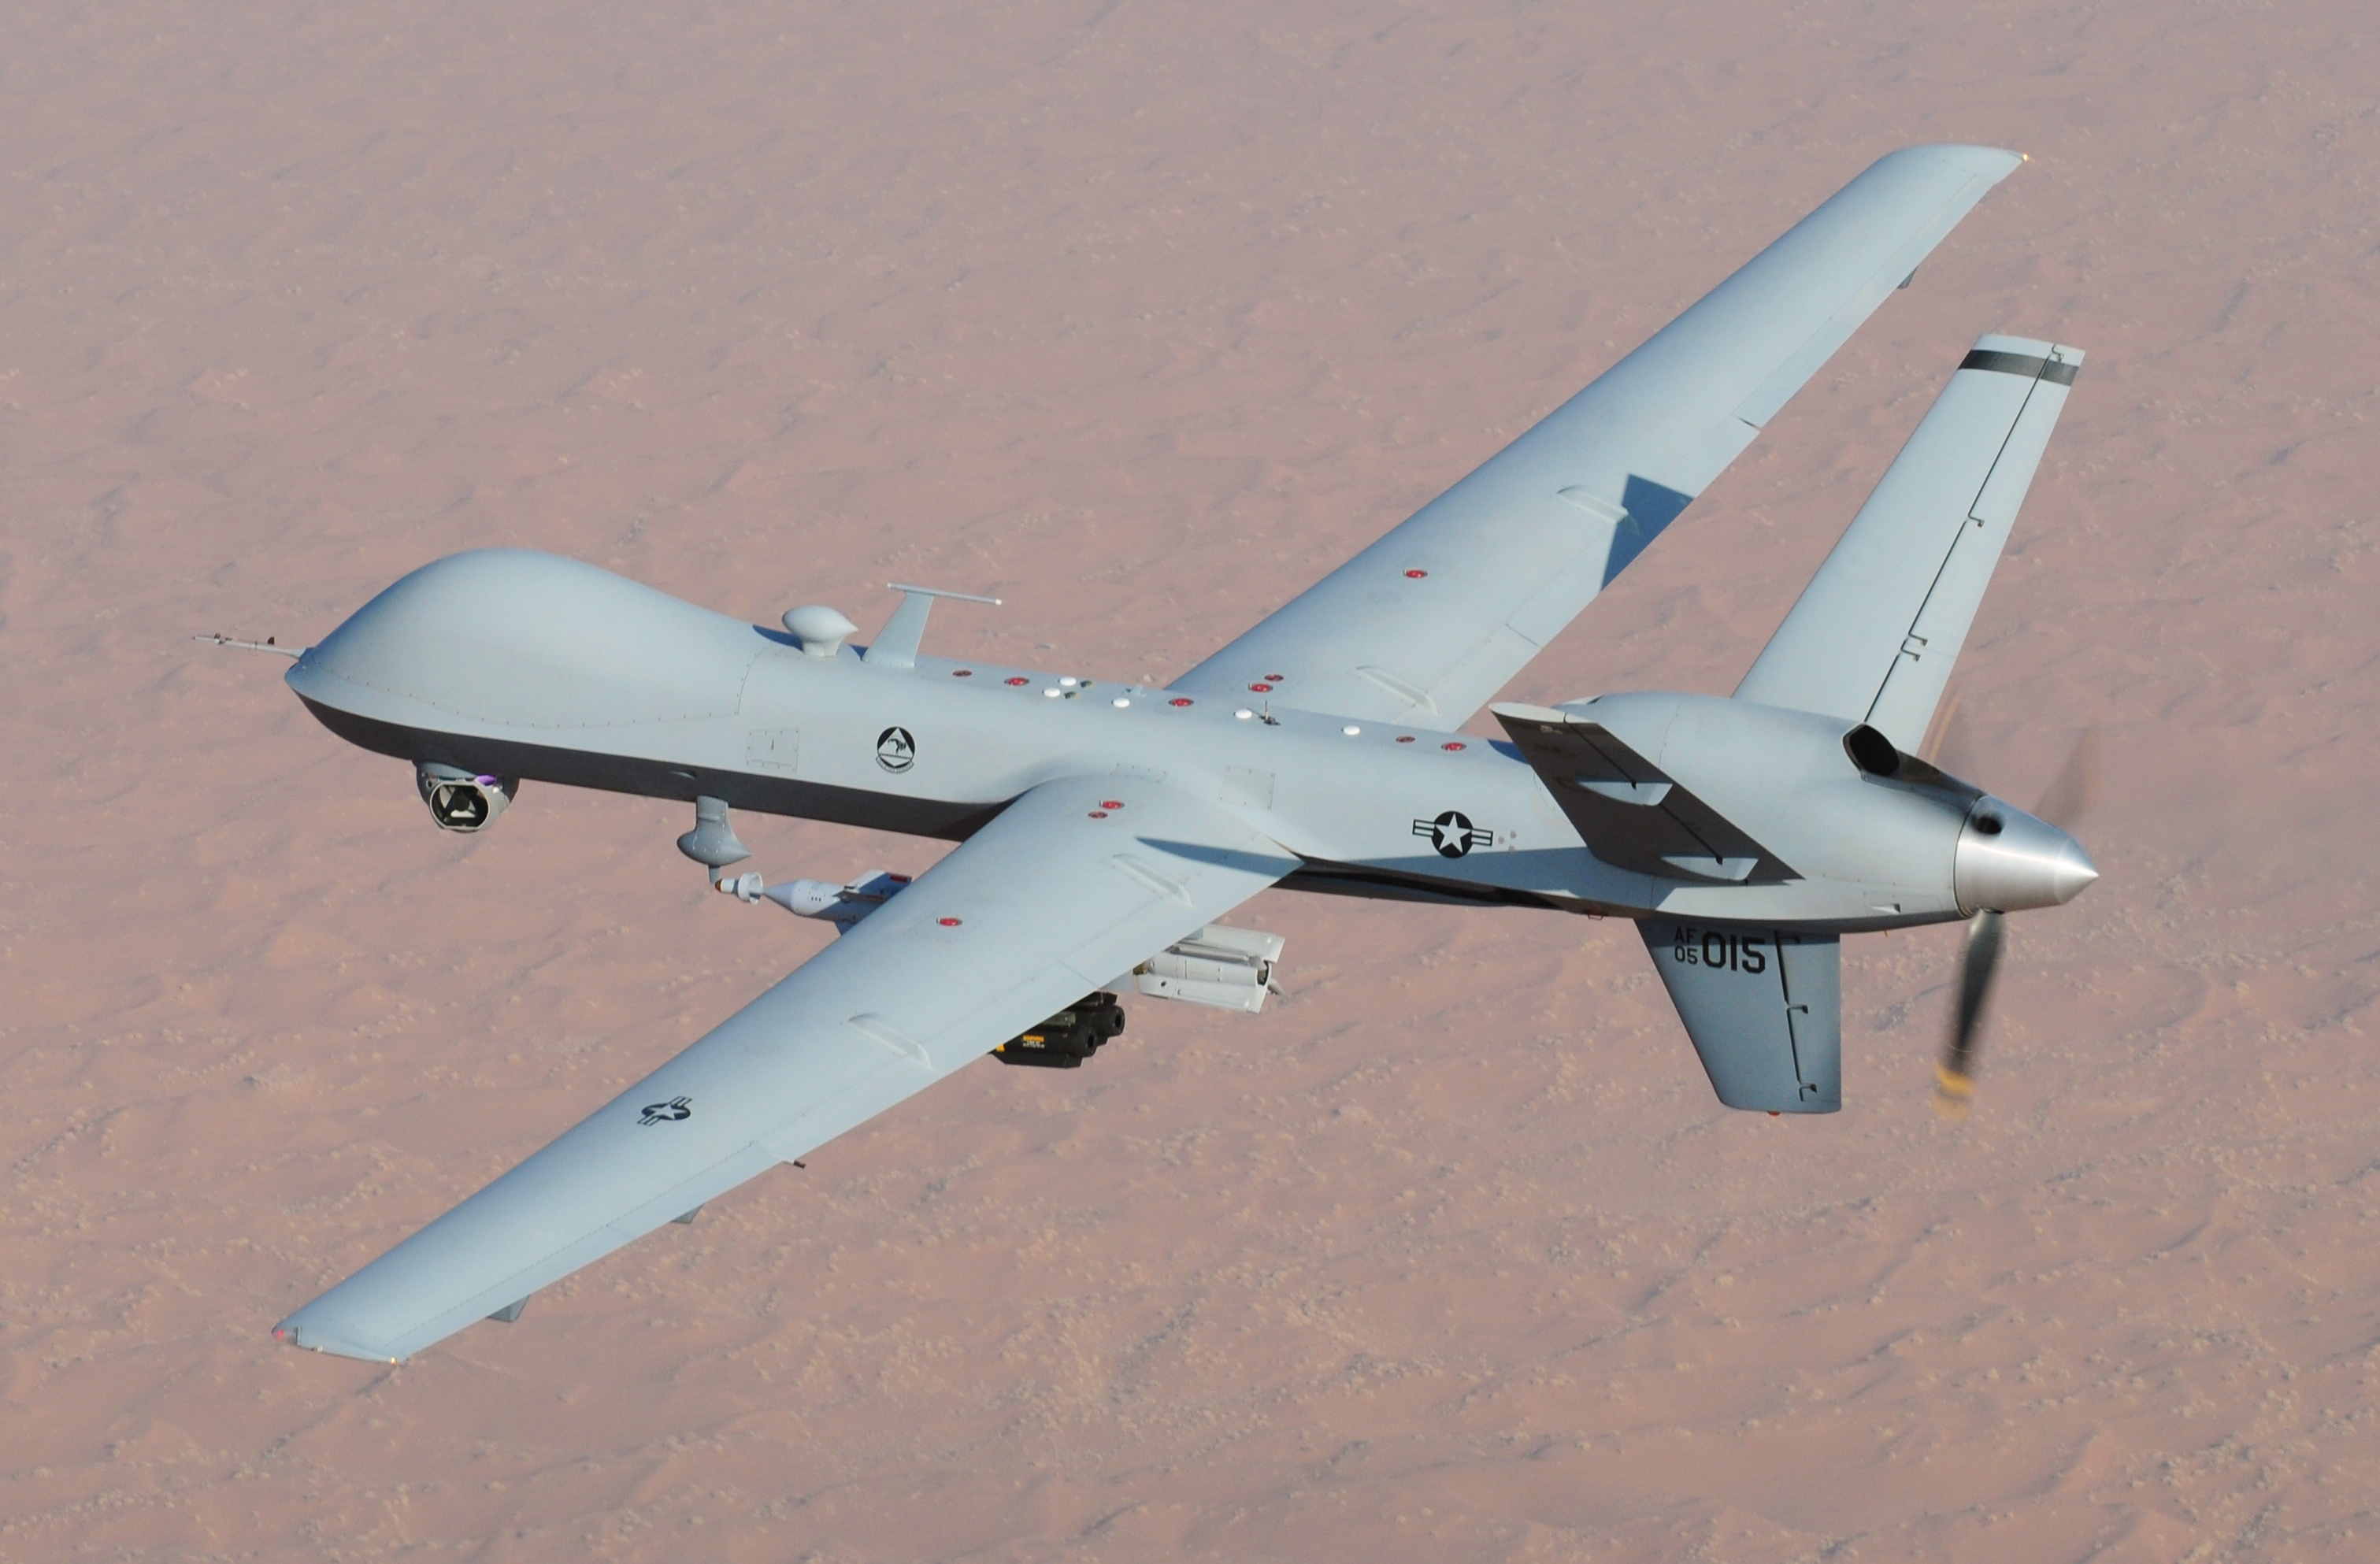
\includegraphics[width=\linewidth]{figs/chap0/MQ-9_Reaper_UAV_(cropped).jpg}
        \caption{MQ‑9 Reaper unmanned aerial vehicle in flight (cropped). Photograph by Lt. Col. Leslie Pratt, U.S. Air Force, 2008, via Wikimedia Commons. Public domain. \cite{mq9_reaper_uav_cropped}}
        \label{fig:spyingQuadcopter}
    \end{subfigure}
    \hfill
    \begin{subfigure}{0.48\textwidth}
        \centering
        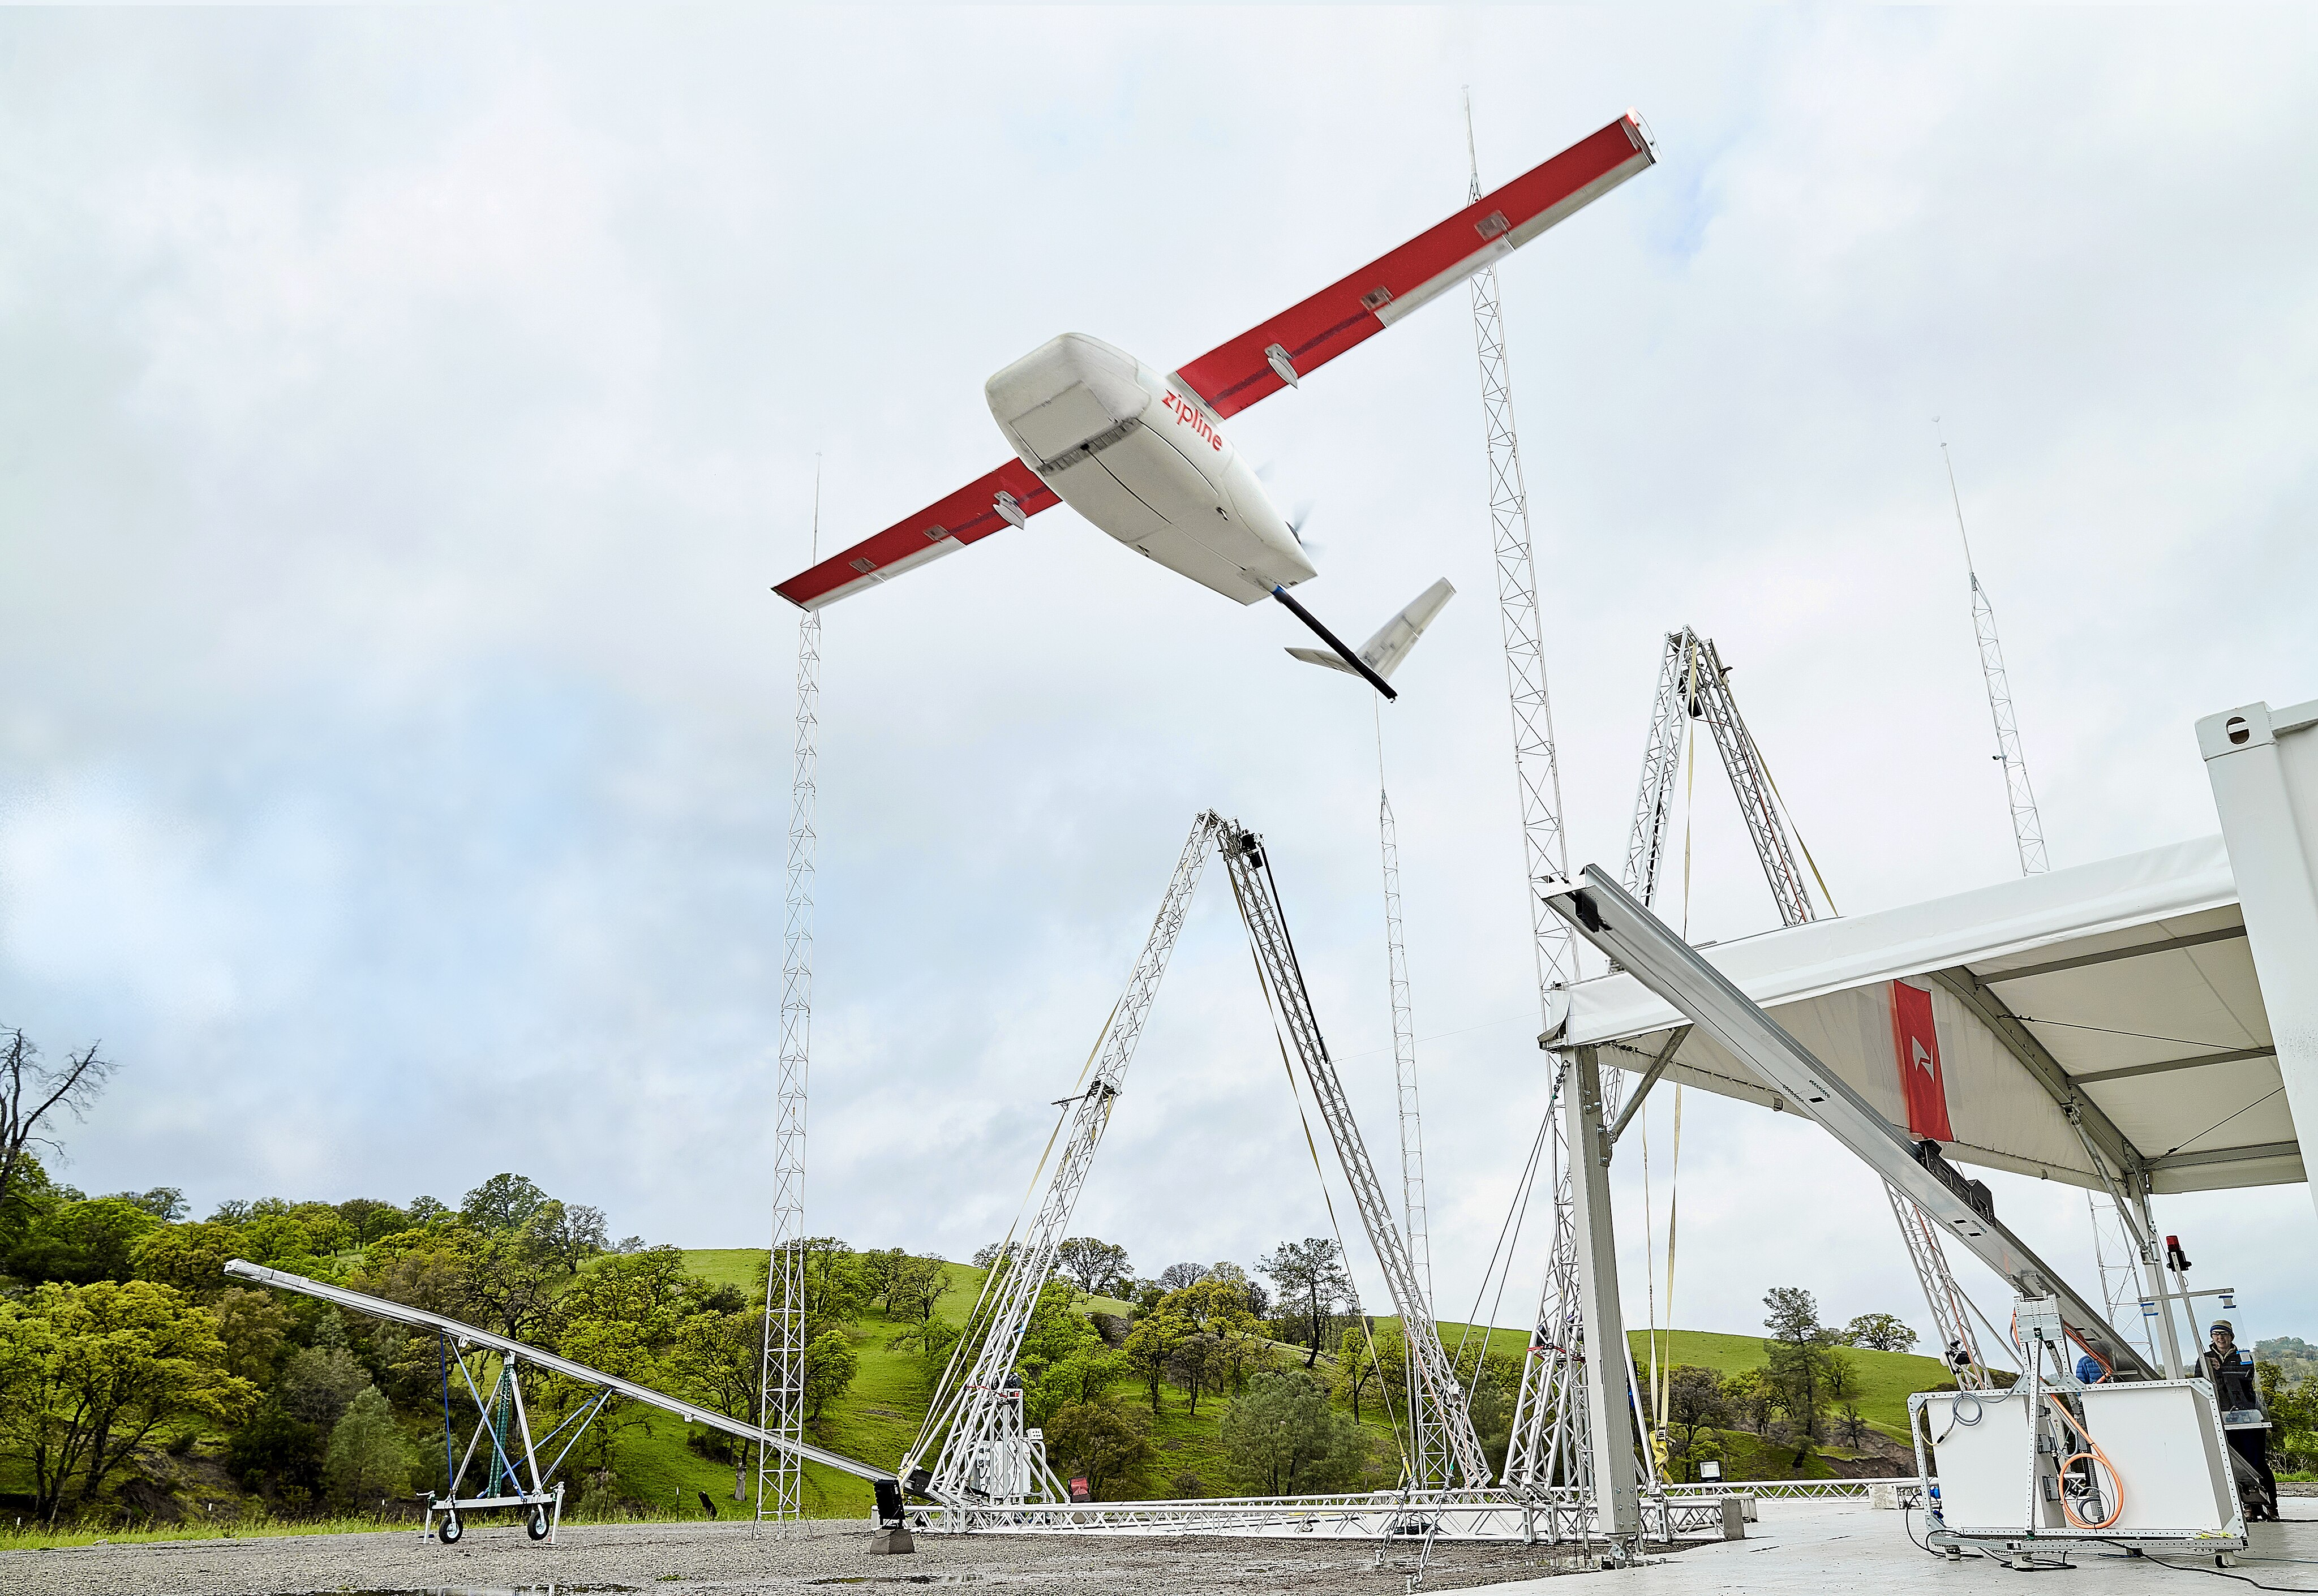
\includegraphics[width=\linewidth]{figs/chap0/4096px-Zipline_Drone_Launch.jpg}
        \caption{Zipline delivery drone launching from its deployment system. Photograph by Zipline, Inc., 2020, via Wikimedia Commons. Licensed under Creative Commons Attribution-ShareAlike 4.0 International (CC BY-SA 4.0). \cite{zipline_drone_launch}}
        \label{fig:ziplineVTOL}
    \end{subfigure} 
    
    \caption{Two Fixed Wing UAVs. The General Atomics MQ9 Reaper (left). Zipline Platform 1 remote delivery aircraft during takeoff (right)}
    \label{fig:FixedWings}
\end{figure}

Today, aircraft are rarely flown manually by a direct remote control pilot. While manual control is fun for recreational purposes, it is hardly accurate or stable enough for many of the missions performed by UAVs. Most aircraft are now flown autonomously using autopilot stacks on the onboard computers. Many open source autopilots exist today, including Px4, Ardupilot, and Rosflight. Two books on writing an autopilot stack for airplane and rotorcraft UAVs were written by \citeauthor{uav_book} and heavily influenced the research in this paper \cite{uav_book, vtol_book}.

The primary interest of this research has been to study control for a specific classification of UAV called a VTOL (vertical takeoff and landing) aircraft. A VTOL is defined as an airplane that can take off and land vertically \cite{Rehan_Akram_Shahzad_Shams_Ali_2022}. That is, they are rotorcraft and airplane hybrids, with airfoils to generate lift and vertical rotors to take off and land vertically. Such hybridization of design allows VTOLs to take advantage of the takeoff and landing capabilities of pure rotorcraft, while also having an airfoil to travel long distances quickly and efficiently. Much research and development is already underway for applications in both civilian and defense spaces. Some examples of existing VTOL craft are shown in Fig. \ref{fig:eVTOLExamples}. 

\begin{figure}[htbp]
    \centering
    \begin{subfigure}{0.48\textwidth}
        \centering
        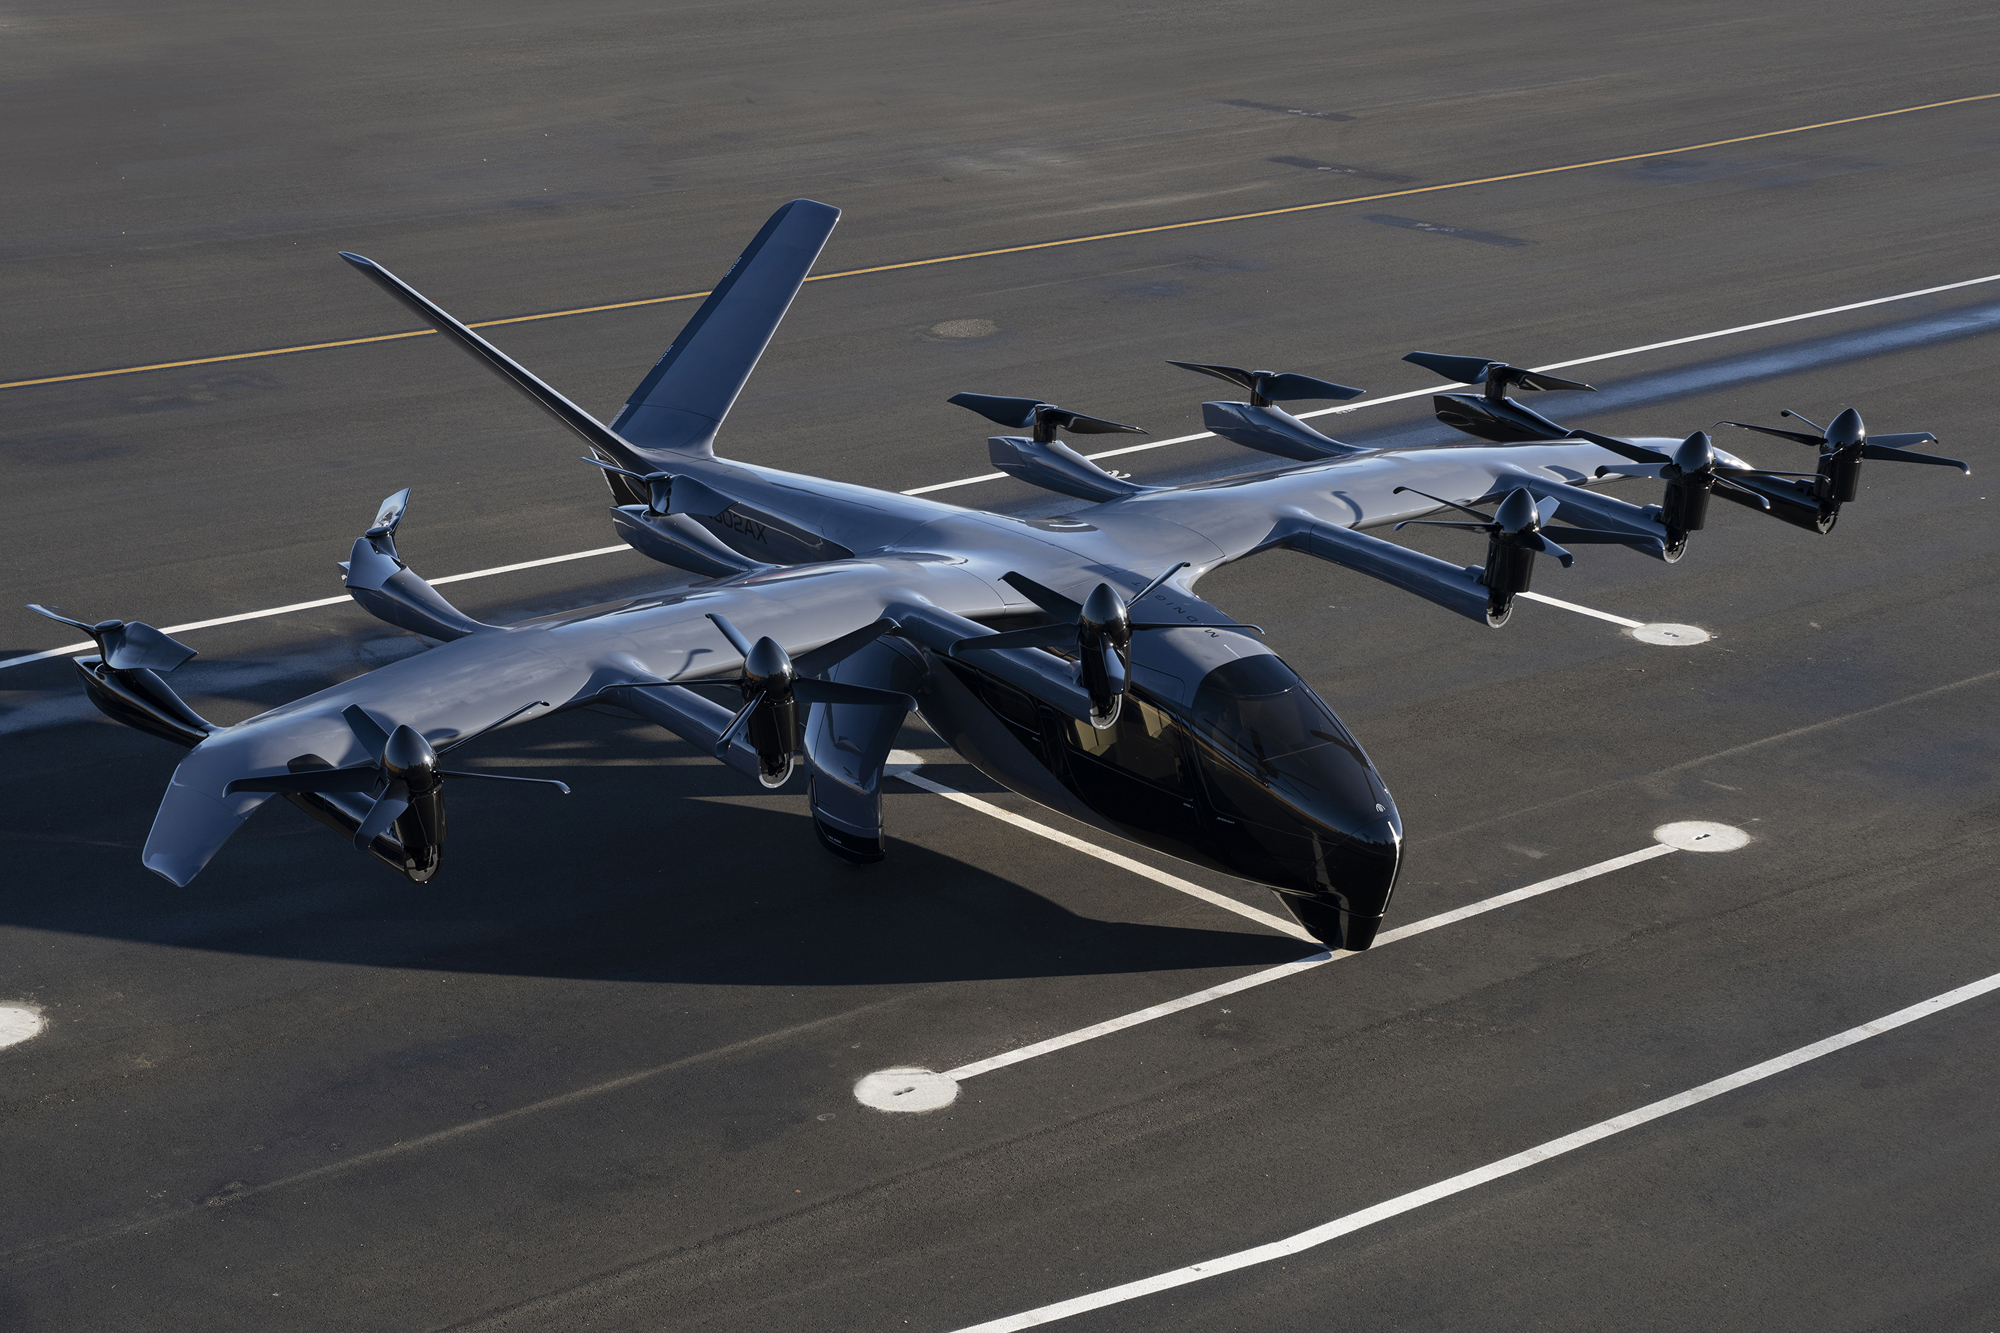
\includegraphics[width=\linewidth]{figs/chap0/Archer_Midnight_top_view.jpg}
        \caption{Archer Aviation Midnight eVTOL prototype aircraft. Image from “Archer Aviation Midnight (production aircraft),” eVTOL News, 2025, \url{https://evtol.news/archer/}. \cite{evtolnews_archer_image}}
        \label{fig:archer}
    \end{subfigure}
    \hfill
    \begin{subfigure}{0.48\textwidth}
        \centering
        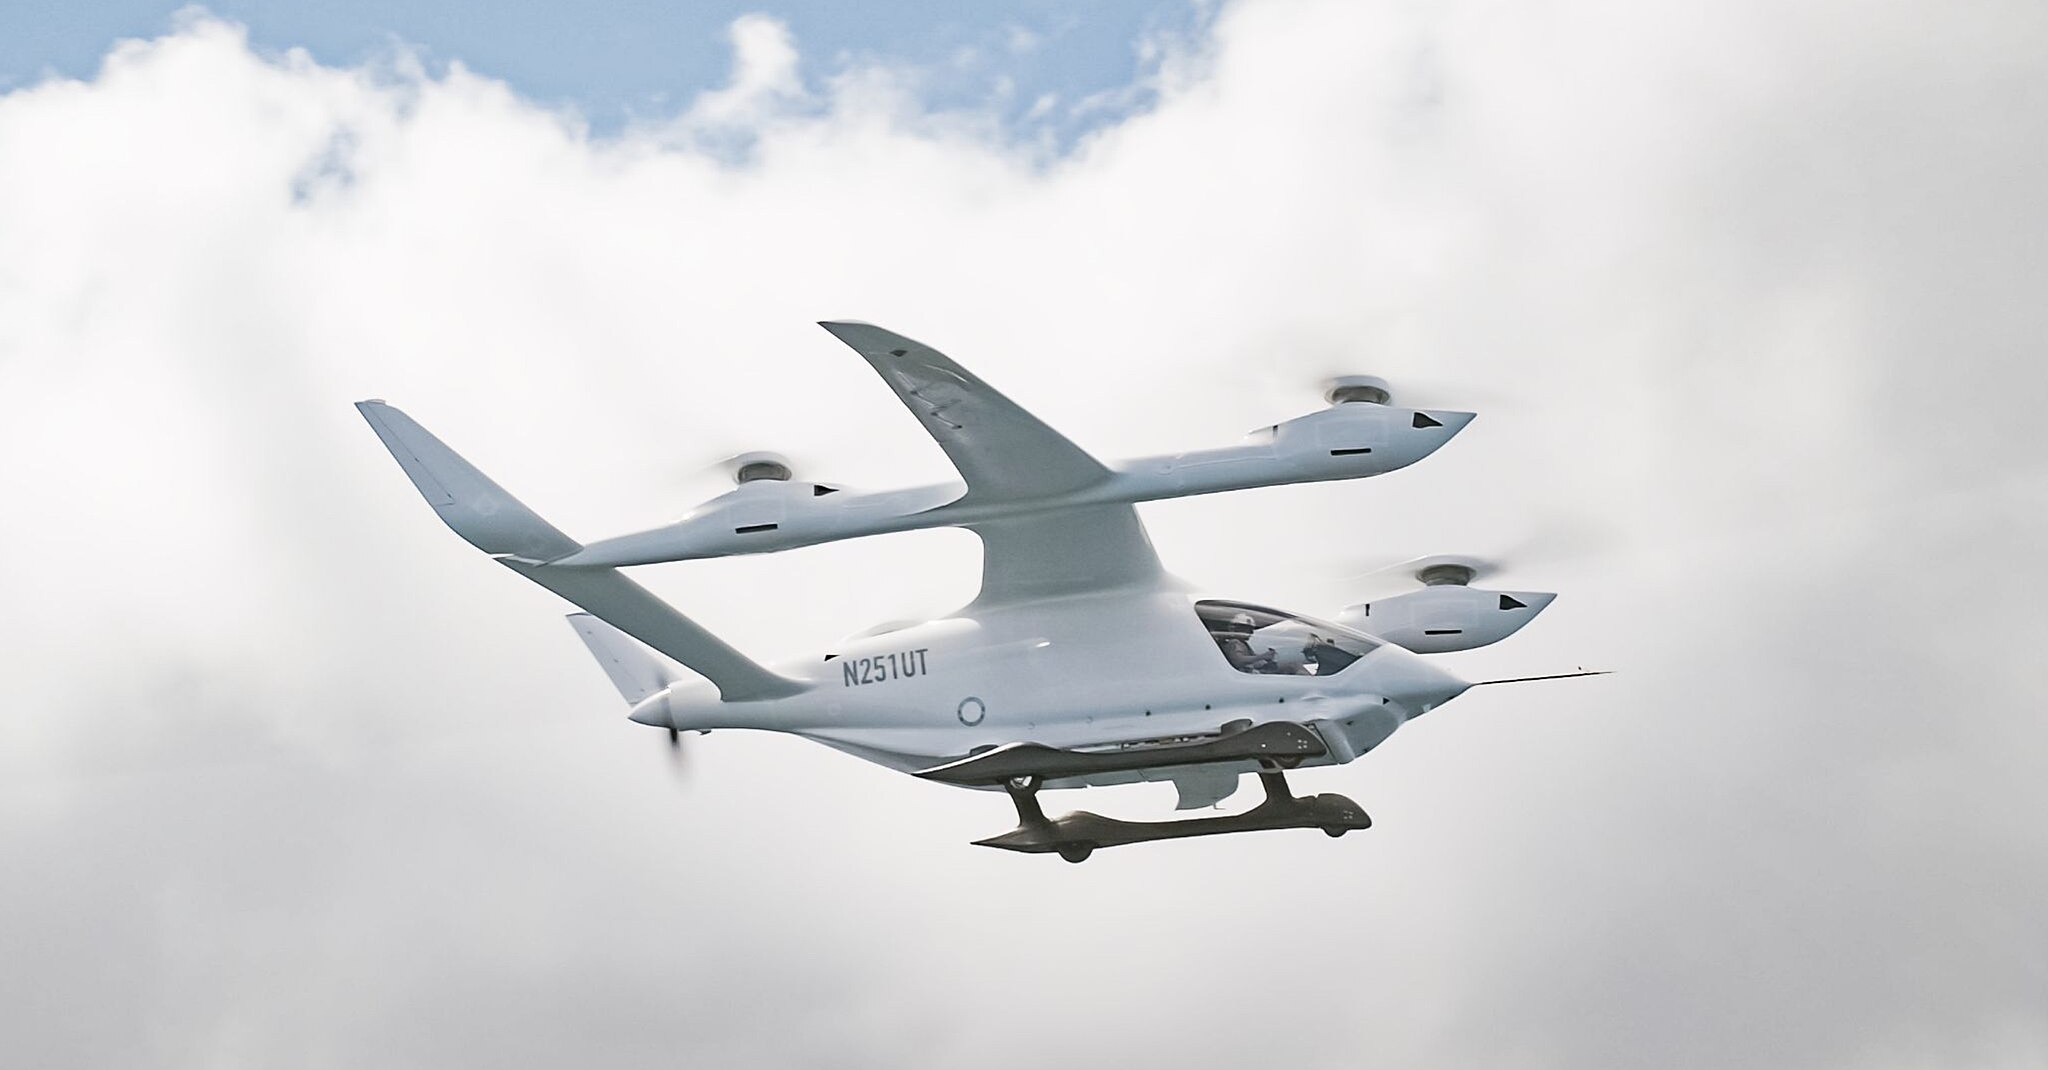
\includegraphics[width=\linewidth]{figs/chap0/2048px-BETA_Technologies_A250_eVTOL_Prototype_Aircraft.jpg}
        \caption{Onyxstar Fox-C8 XT Xender 360 UAV. Image by ZullyC3P (2015), via Wikimedia Commons. Licensed under Creative Commons Attribution-ShareAlike 4.0 International (CC BY-SA 4.0). \cite{beta_a250_evtol_prototype}}
        \label{fig:BetaTech}
    \end{subfigure}

    \vspace{0.5cm}  % vertical spacing between rows

    % Row 2
    \begin{subfigure}{0.48\textwidth}
        \centering
        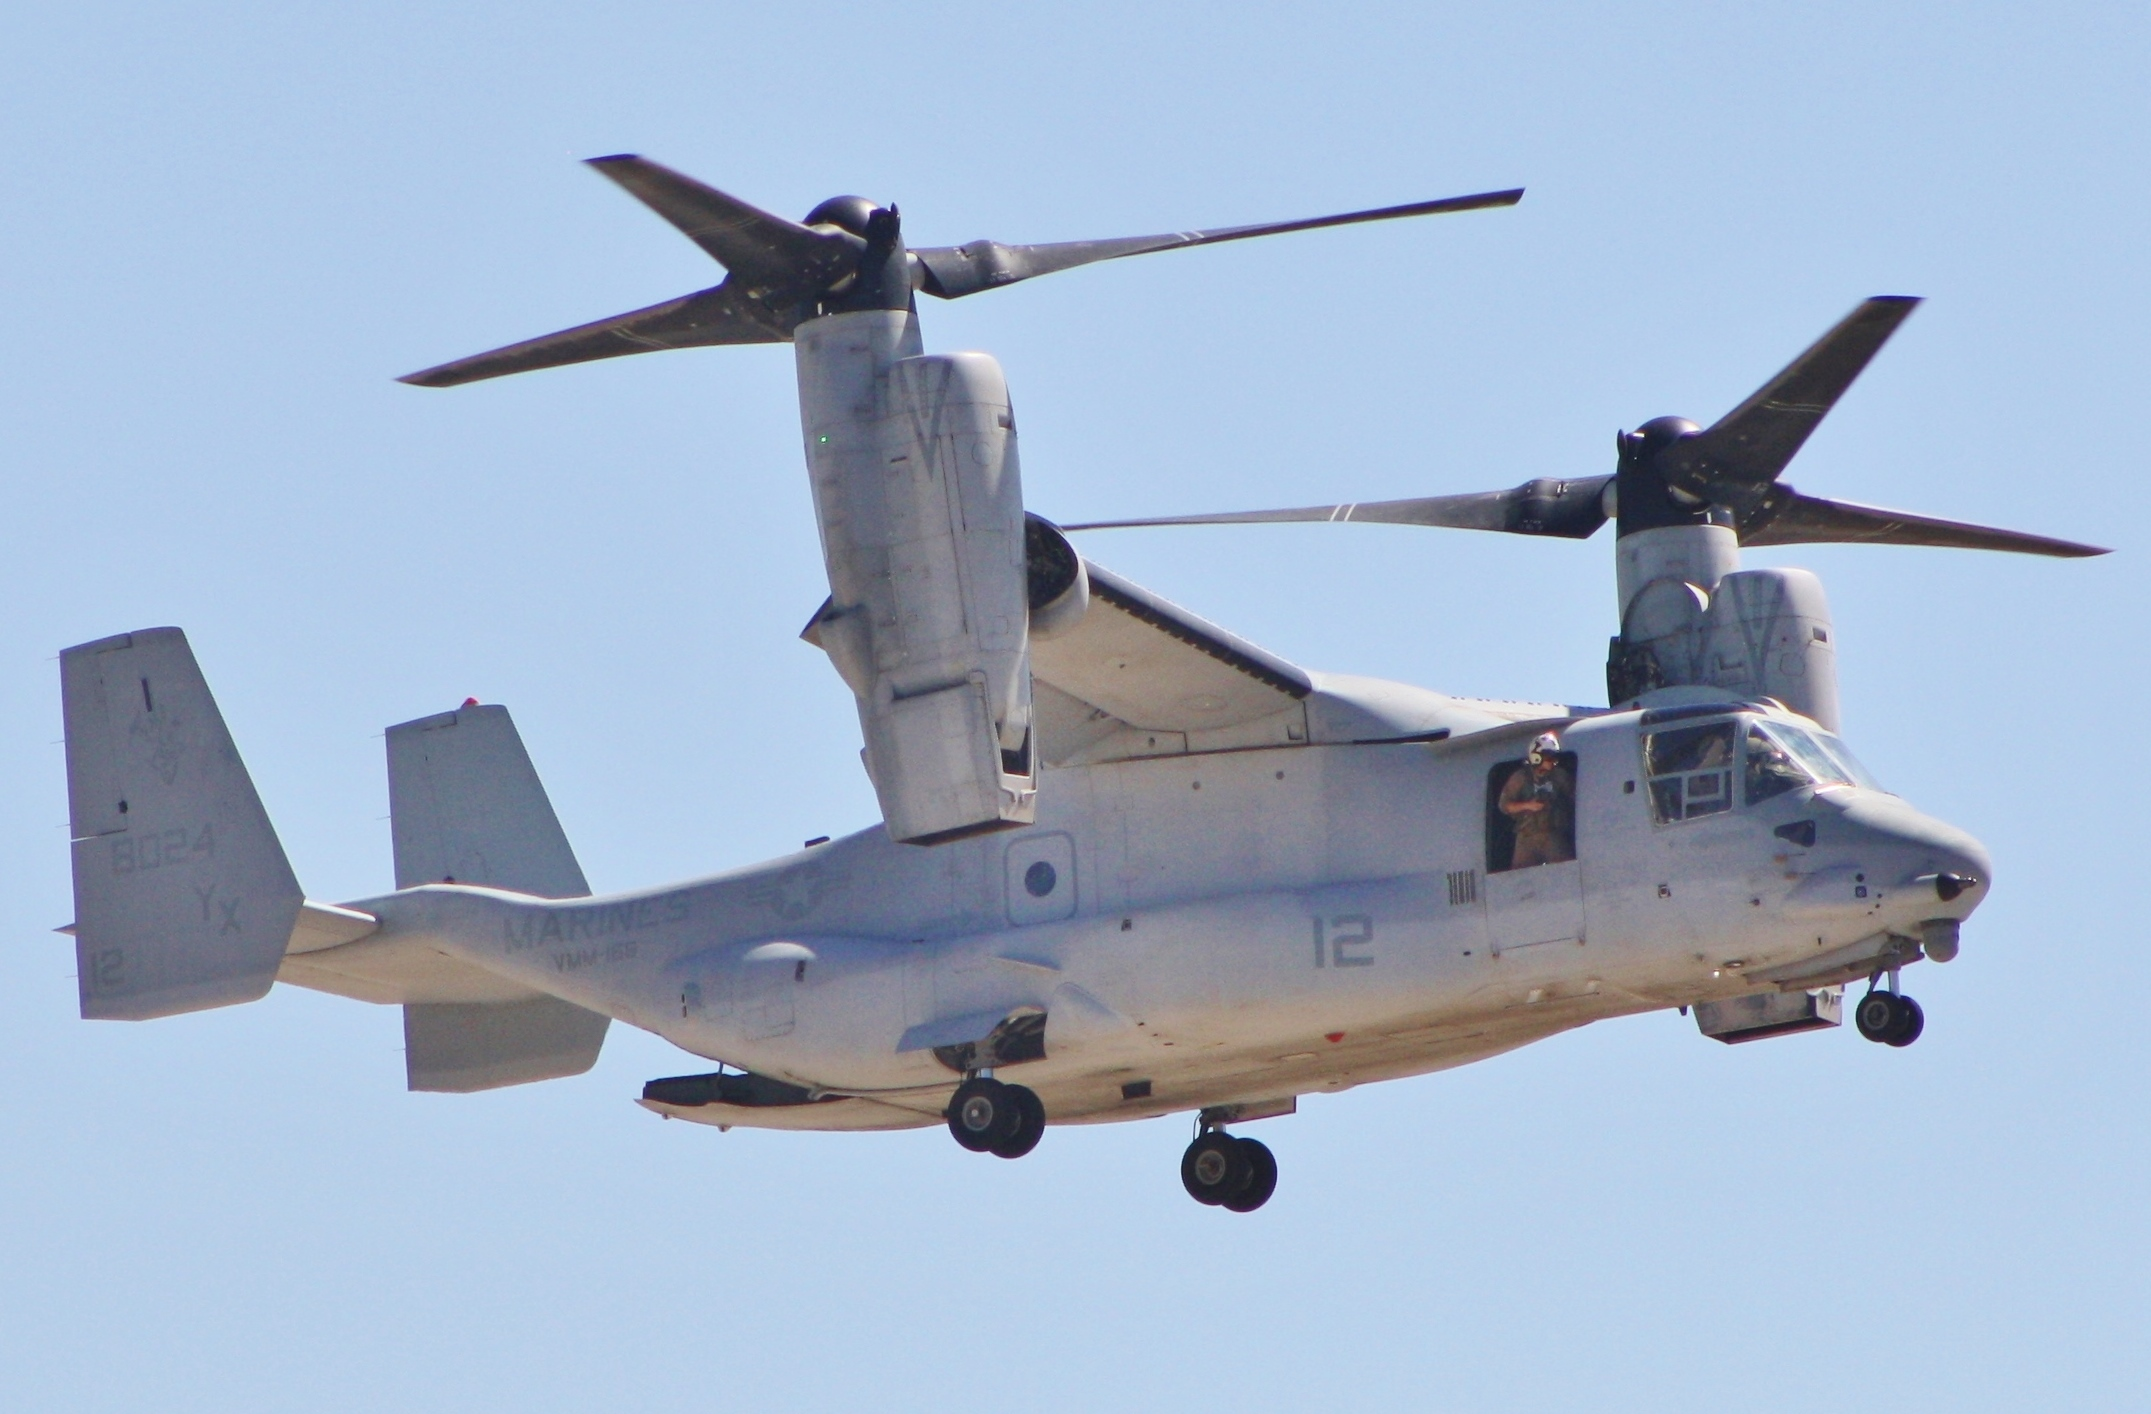
\includegraphics[width=\linewidth]{figs/chap0/MV-22_mcas_Miramar_2014.jpeg}
        \caption{U.S. Marine Corps MV‑22B Osprey tiltrotor aircraft at Marine Corps Air Station Miramar, California, during the 2014 air show. Photograph by FOX 52, 2014, via Wikimedia Commons. Licensed under Creative Commons Attribution‑ShareAlike 4.0 International (CC BY‑SA 4.0). \cite{mv22_mcas_miramar_2014}}
        \label{fig:osprey}
    \end{subfigure}
    \hfill
    \begin{subfigure}{0.48\textwidth}
        \centering
        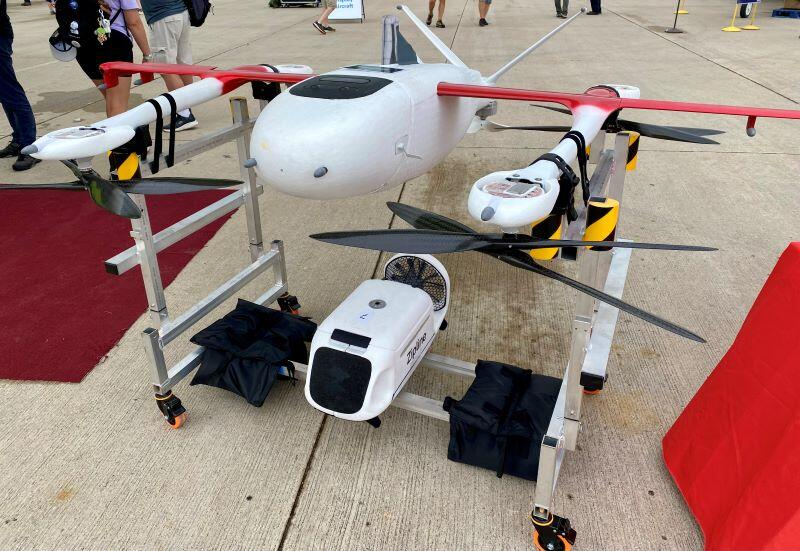
\includegraphics[width=\linewidth]{figs/chap0/zipline_source_bill_carey.jpg}
        \caption{Zipline second‑generation P2 autonomous delivery drone on display at EAA AirVenture Oshkosh. Photograph by Bill Carey for Aviation Week Network, 2024, from “Zipline Exhibits 2nd Generation P2 Drone,” Aviation Week Network \cite{zipline_p2_drone_aviationweek}}
        \label{fig:zipline}
    \end{subfigure}    
    
    \caption{Four different commercial and defense eVTOL aircraft in various stages of development and use. Each design is specialized to the use case and developer's design philosophy. Figs. \ref{fig:archer} and \ref{fig:BetaTech} are commercial eVTOL air taxis in development from Archer Aviation and Beta Technologies, respectively. The V-22 Osprey in Fig. \ref{fig:osprey} is a famous VTOL that has seen extensive use by the U.S. Military. Fig. \ref{fig:zipline} is the Zipline VTOL, which is under development for food and package delivery.}
    \label{fig:eVTOLExamples}
\end{figure}

The most difficult challenge for VTOL control is transitioning. Transition refers changing from rotorcraft hovering flight into airframe forward flight and vice versa. The goal for a transition autopilot is to take the aircraft from hover to forward flight and back again as quickly, efficiently, and stabily as possible. During takeoff transition, the aircraft needs to slowly gain altitude while simultaneously gaining forward airspeed to generate more lift, while the opposite is true for landing. Unfortunately, during the transision, the aircraft is subject to uncertain dynamics and conditions that hold for neither mode of control. For example, angle of attack $\alpha$ is often far larger than permissible for a standard airplane controller. This makes it impossible to use a purely standard control law. 

A problem with many current solutions is that they bifurcate the transition of aircraft into multiple parts. In other words, aircraft are only thought of as fixed-wing aircraft or multicopter aircraft, and that an aircraft can only be one of those at a given time. In other words, when the VTOL aircraft is moving at low lateral airspeed, it is considered to actually be a multicopter and thus uses a multicopter autopilot framework. Likewise, when the aircraft is moving at a high lateral airspeed, the aircraft is considered to be a fixed-wing airplane with a fixed-wing autopilot framework. This mentality leads to a bifurcation in autopilot design; both fixed-wing and quadrotor control are excellent in their own domains, but their isolation from each other causes significant issues in bridging between the two. 

In addition to the VTOL controller, several other tangential areas for control and planning were explored and developed.
First, during the first stages of development of the VTOL controller, it became apparent that the controller would be model dependent.
In particular, we desired to obtain the aerodynamic coeffients for the vehicle.
There was no 3D CAD model of the first VTOL aircraft being developed, so it was not feasible to use aerodynamic software to determine a model for the aircraft.
However, real flight data was and is readily accessible to the user after a fixed-wing flight.
Therefore, a system identification scheme was developed that used flight data with an assumed system structure to recursively estimate the coefficients of aerodynamics.
This system identification scheme was implemented for a fixed-wing simulation successfully identified the majority of coefficients of aerodynamics for the vehicle.

The 2D VTOL quadplane controller requires a reference trajectory to be followed by the quadplane.
This reference trajectory must include a reference position, velocity, and acceleration; each of these references are required for the VTOL to function.
$3^{rd}$ degree basis splines (B-Splines) intrinsically include $1^{st}$ and $2^{nd}$ derivatives, which are easily calculated due to their polynomial composition; therefore $3^{rd}$ degree uniform B-Splines were used for the entirety of this paper to represent reference position.
Due to their practical applications, it is desired to generate B-Splines as quickly and computationally efficiently as possible.
In order to facilitate this, a set of look up tables were created to efficiently generate a particular class of B-Splines trajectories, called minimum snap trajectories.
In the implementation developed here, the control points that define a minimum-snap trajectory are generated using stored data in lookup tables.
That data is then accessed and combined to generate the control points for the desired trajectory.

However, this method is not able to account for obstacles in the environment. 
The final contribution of this paper is a path planning algorithm that avoids obstacles and generates a B-Spline trajectory between a start and end point.
This path planning method uses the Rapidly Exploring Random Trees (RRT) algorithm to generate a safe set of spaces or corridors between start and end points.
Within this set of corridors a $3^{rd}$ degree B-Spline is generated as the actual flight path between start and end points.
This algorithm further facilitates the generation of smooth paths without intersection of obstacles.

Each of these components are part of the growing framework for the development of unmanned aerial robotics systems.

\subsection{Contributions}

\begin{itemize}
    \item Differentially flat 2D quadplane controller
    \item Aerodynamic coefficient system identification
    \item B-Spline look up tables for minimum snap trajectory generation
    \item Obstacle avoidance path planner using safe flight corridors and an optimized B-Spline path
\end{itemize}

